\section{Deep Reinforcement Learning 1 (Use Deep RL)}
\subsubsection*{Goal}
\begin{itemize}
    \item Which algorithm to take
    \item Which framework do exist
    \item Which hyperparameter are most important to get right first
    \item How to design environment and rewards
\end{itemize}
\subsection{Frameworks}
\subsubsection*{OpenAI gym / gymnasium}
\begin{itemize}
    \item Not really a framework for RL Algorithms, but for the \textbf{environment}
    \item Many other frameworks use the gym environment model or build upon the same interface
    \item Contains useful utilities and wrappers
    \item Contains many standard benchmark environments
\end{itemize}
\subsubsection*{Stable Baseline 3}
\begin{itemize}
    \item Contains reliable implementation of basic RL algorithms
    \item Relative beginner friendly
    \item Less efficient and parametrized than other frameworks
\end{itemize}
\subsubsection*{RLLIB on Ray}
\begin{itemize}
    \item Large collection of algorithms
    \item Able to provide own implementation of models and algorithms
    \item Builds upon ray and ray.tune for distributed workflows
    \item More advanced and difficult to use (or debug)
    \item Our framework of choice for research problems that require complex algorithms and days of training
\end{itemize}
\subsubsection*{Spinning up}
Educational resource to make it easier to learn RL.

\subsection{Optimizing Deep Q-Learning}
Training for Deep Q-Learning is often difficult; several further concepts have been developed to make training easier:
\begin{itemize}
    \item \textbf{Prioritized Experiance Replay}
    \item \textbf{Double Q-Learning}
    \item \textbf{Dueling Networks}
    \item Multi-step boostrap target
    \item Distributional DQN
    \item Noisy DQN
    \item \textbf{Target weights updates}
\end{itemize}

\subsubsection{Prioritized Experiance Replay}
Idea:
\begin{itemize}
    \item An agent should be able to learn more efficiently from transitions than from others
    \item By what criterion can we measure the importance of each transition
\end{itemize}
\textbf{TD error} indicates how surprising or unexpected the transition is, so samples with a high TD error should be prioritizd.
However:
\begin{itemize}
    \item Only using the prioritized transition can lead to errors too 
    \item Use stochastic sampling and the priority as weights for the probability
\end{itemize}
\subsubsection*{Calculating Priorities}
Calculate Priorities from TD Errors:
\begin{itemize}
    \item Take the magnitude of the TD Error as Priority
    \item Store the priorities with each corresponding tuple in the replay buffer
    \item Compute sampling probabilities when creating the batches
\end{itemize}
TD Error is Zero:
\begin{itemize}
    \item If the TD Error is zero, the priority will also be zero
    \item To prevent tuples from starving, we can add a small constant
    \[
    p(i) = |\delta_i| + epsilon
    \]
\end{itemize}
\subsubsection*{Prioritized Experience Replay: Sampling}
The probability of sampling a transition \(i\) is
\[
P(i) = \frac{p_i^\alpha}{\sum_{k}^{}p_k^\alpha}
\]
the parameter \(\alpha\) is another hyperparameter that controls the influence of priority values:
\begin{itemize}
    \item if it is equal to 0, the priorities are ignored, and uniform sampling is used
    \item if it is 1, only the priorities are used
\end{itemize}

\subsubsection{Double Q-Learning}
\begin{itemize}
    \item Q-Learning is known to overestimate action-values under certain conditions
    \item The Q function is used in both to \textbf{select the best action} and to \textbf{evaluate} it:
    \[
    y_j^{DQN} = R_j + \gamma Q(S_{j+1},\text{arg}\max_a Q(S_{j+1},a,\boldsymbol{w}),\boldsymbol{w})
    \]
    \item In the early stages of learning, the Q function can be noisy, then a possible wrong Q value can be increased too much
    \item Overestimating can be diminished by using a second function approximation:
    \[
    y_j^{DoubleDQN} = R_j + \gamma Q(S_{j+1},\text{arg}\max_a Q(S_{j+1},a,\boldsymbol{w}),\boldsymbol{w}')
    \]
    \item now the value is only increased if the Q value is high in both approximations
    \item Where do we get another function approximation from?
    \item In DQN we already use two networks and \(w^-\) is significantly different enough from \(w\) to be used:
    \[
    y_j^{DoubleDQN} = R_j + \gamma Q(S_{j+1},\text{arg}\max_a Q(S_{j+1},a,\boldsymbol{w}),\boldsymbol{w}^-)
    \]
\end{itemize}
\subsubsection{Dueling Networks}
The idea behind dueling networks is to use a \textbf{two-headed} network that branches into head each for calculating:
\begin{itemize}
    \item The \textbf{value} function
    \item The \textbf{advantage} function
    \item The sum of the two function will give the action-value function, as
    \[
    Q(s,a) = V(s) + A(s,a)
    \]
\end{itemize}
\begin{figure}[!h]
    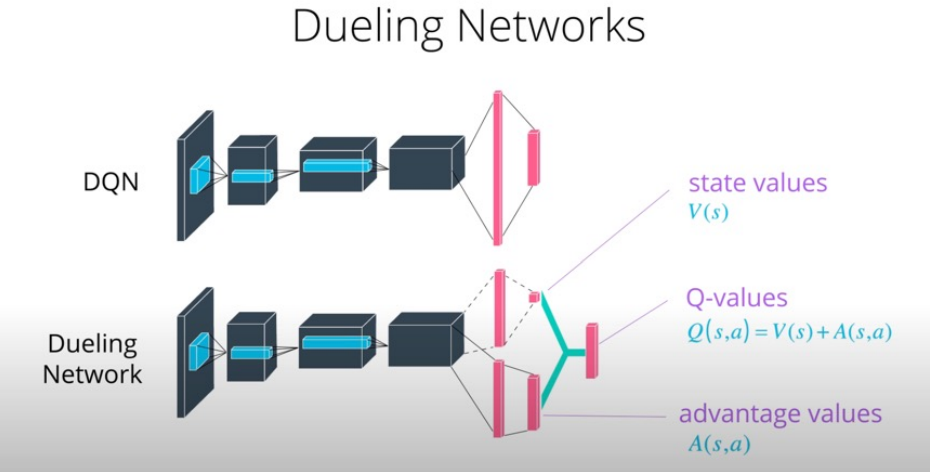
\includegraphics[width = \columnwidth]{figures/DeepReinforcementLearning3/DuelingNetworks.png}
\end{figure}
\subsubsection{Update of target weights}
A different set of weights are used for the target function on DQN, than the one that is trained.
This set must be updated with the trained version.

Update strategie:
\begin{itemize}
    \item Update after n training steps (original DQN)
    \item Update by linear interpolation between target and current weights (often works better)
    \[
    w^- = \tau w + (1-\tau)w^-
    \]
\end{itemize}
\subsubsection{Trust Region Policy Optimization (TRPO)}
In policy gradient methods, the update is calculated as
\[
\boldsymbol{\theta}_{t+1} = \boldsymbol{\theta}_t + \alpha\nabla J(\boldsymbol{\theta})|_{\boldsymbol{\theta} = \boldsymbol{\theta}_t}
\]
The new values for \(\theta\) should be near to the old values, as we use a small step size, however, the \textbf{policy} could still change significantly with a change of \(\boldsymbol{\theta}\).

We would like to make sure that the \textbf{new and old policies} are not too far apart (not that only the parameters are close)
\subsubsection*{Trust Region Policy Optimization}
\begin{itemize}
    \item We would like to compare the policies, but these are distributions (probabilities for each action)
    \item We can use the Kullback-Leiber divergence (KL-divergence), this is a common measure to compare distributions
    
    \[
    D_{KL}(P||Q) = \sum_{x}^{}P(x) \text{log}\frac{P(x)}{Q(X)}
    \]
\end{itemize}

We can write the cost function as a function of two policies and optimize that
\[
J(\boldsymbol{\theta},\boldsymbol{\theta}_t) = \mathbb{E}_{a~\pi}\left[\frac{\pi_{\boldsymbol{\theta}}(a|s)}{\pi_{\boldsymbol{\theta}_t}(a|s)}A(s,a)\right]
\]
i.e. this measures how the new policy performs relative to the old policy, then we find 
\[
    \boldsymbol{\theta}_{t+1} = \text{arg}\max_{\boldsymbol{\theta}} J(\boldsymbol{\theta},\boldsymbol{\theta}_t)
\]
under the constrained
\[
D_{KL}(\boldsymbol{\theta}_{t+1}||\boldsymbol{\theta}_t) \le \delta
\]
\begin{itemize}
    \item So we maximize the so-called surrogate performance function:
    \[
    J(\boldsymbol{\theta},\boldsymbol{\theta}_t)
    \]
    \item Actual implementation is mathematically a bit more complicated
    \item A Taylor approximation of the objectiv and the constraint is used
    \item As this approximation requires to inverse a matrix (which is very expensiv for the many parameters of a neural network), the constraint problem of optimization is solved by approximate solutions (conjugate gradient)
    \item The idea behind TRPO and using the surrogate performance functions are good, but tha algorithm is inefficient \(\rightarrow\) PPO
\end{itemize}
\subsubsection{Proximal Policy Gradient (PPO)}
\begin{itemize}
    \item PPO tries to solve the same problem but uses clipping instead of constraint on the KL-divergence
    \item Enforcing a constraint can also be viewed as imposing a penalty when the function gets near to it
    \item So there are two variants of PPO, with clippingor with a penalty
    \item We will show a deriviation of PPO from the additional viewpoint of trajectory sampling
\end{itemize}
\subsubsection*{Policy Update in REINFORCE}
\begin{figure}
    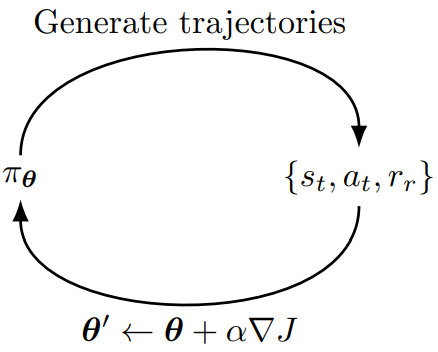
\includegraphics[width = 0.5\columnwidth]{figures/DeepReinforcementLearning3/PPOPolicyUpdate.png}
\end{figure}
\begin{itemize}
    \item The policy is used to generate a trajectory (episodes or part of one)
    \item The trajectory is then used to calculate the gradient and update the policy
    \item So, the just sampled trajectories do not correspond to actual policy
    \item Sampling trajectories is computing intensive: Could we recycle old trajectories?
\end{itemize}
\subsubsection*{Importance Sampling}
To calculate any experience values, we need to incorporate the probability of the trajectory:
\begin{equation*}
    \sum_{\tau}^{}P(\tau;\boldsymbol{\theta}')R(\tau)
\end{equation*}

\begin{equation*}
    \sum_{\tau}^{}P(\tau;\boldsymbol{\theta})\frac{P(\tau;\boldsymbol{\theta}')}{P(\tau;\boldsymbol{\theta}')}R(\tau)
\end{equation*}
\(P(\tau;\boldsymbol{\theta})\) is the old policy.
\(\frac{P(\tau;\boldsymbol{\theta}')}{P(\tau;\boldsymbol{\theta}')}R(\tau)\) is the Re-weight factor.
So we can use old trajectories if we weight the sample according to the re-weighting factor.
\subsubsection*{Re-weighting factor}
\[
\frac{P(\tau;\boldsymbol{\theta}')}{P(\tau;\boldsymbol{\theta})} = \frac{
    \pi_{\boldsymbol{\theta}'}(a_1|s_1) \pi_{\boldsymbol{\theta}'}(a_2|s_2) \pi_{\boldsymbol{\theta}'}(a_3|s_3) \dots
}{
    \pi_{\boldsymbol{\theta}}(a_1|s_1) \pi_{\boldsymbol{\theta}}(a_2|s_2) \pi_{\boldsymbol{\theta}}(a_3|s_3) \dots
}
\]
\begin{itemize}
    \item Can easily be close to zero or infinity if any of the policies become close to 0
    \item We would like to ensure that this factor remains close to 1
\end{itemize}
\subsubsection*{Re-weighting Policy Gradient}
\begin{equation*}
        g = \underbrace{\nabla_{\boldsymbol{\theta}'}\sum_{t}^{}\frac{
    \pi_{\boldsymbol{\theta}'}(a_t|s_t)
    }{
    \pi_{\boldsymbol{\theta}}(a_t|s_t)
    }R_t}_{L_{sur}}
\end{equation*}
\begin{equation*}
    g = \nabla_{\boldsymbol{\theta}'}L_{sur}(\boldsymbol{\theta}',\boldsymbol{\theta})
\end{equation*}
\begin{equation}
    L_{sur}(\boldsymbol{\theta}',\boldsymbol{\theta}) = \nabla_{\boldsymbol{\theta}'}\sum_{t}^{}\frac{
        \pi_{\boldsymbol{\theta}'}(a_t|s_t)
        }{
        \pi_{\boldsymbol{\theta}}(a_t|s_t)
        }R_t
\end{equation}
This is only valid, if the old and the new policy is similar.

\subsubsection{PPO: Clipped Objective}
CPI: Conservative Policy Iteration 
\begin{equation*}
    L^{CPI}(\boldsymbol{\theta}) = \mathbb{E}_t\left[\frac{
        \pi_{\boldsymbol{\theta}}(a_t,s_t)
        }{
            \pi_{\boldsymbol{\theta}(a_t|s_t)}
        }A_t\right] = \mathbb{E}_t\left[r_t(\boldsymbol{\theta})A_t\right]
\end{equation*}
\begin{equation*}
    L^{CLIP} = \mathbb{E}_t\left[
        \min(r_t(\boldsymbol{\theta})A_t,clip(r_t(\boldsymbol{\theta}),1-\epsilon,1+\epsilon))
    \right]
\end{equation*}
\begin{equation*}
    \boldsymbol{\theta}_{k+1} = \text{arg}\min_{\boldsymbol{\theta}}\mathbb{E}_t\left[
        \min(r_t(\boldsymbol{\theta})A_t,clip(r_t(\boldsymbol{\theta}),1-\epsilon,1+\epsilon))
    \right]
\end{equation*}
\begin{figure}[!h]
    \centering
    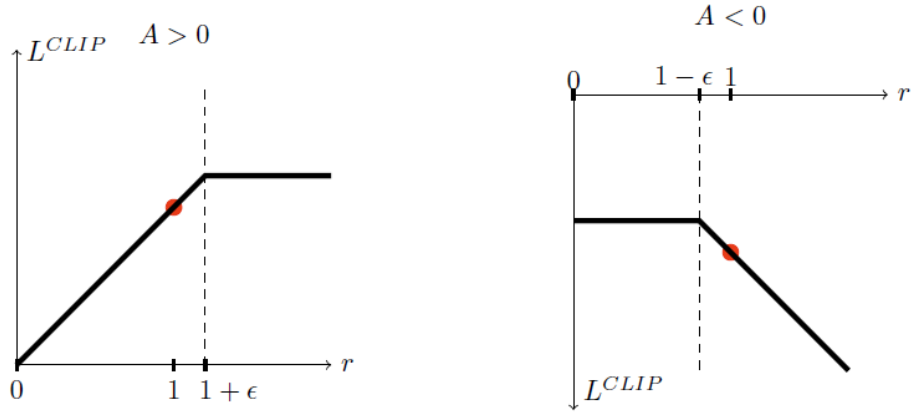
\includegraphics[width = 0.5\columnwidth]{figures/DeepReinforcementLearning3/PPOClip.png}
\end{figure}
\subsubsection*{PPO Summary}
\begin{itemize}
    \item By adjusting the step size in the update of the weights, we can ensure that the weights do not change too much
    \item However, even a small change in the weights could be a large change in the policy
    \item We would like to ensure, that the policy does not change too much
    \item In PPO, we enforce that the ratio of the new to old policy stays within 
    \[
    \left[1-\epsilon,1 + \epsilon\right]
    \]
\end{itemize}
\subsection{Asynchronous Advantage Actor-Critic (A3C)}
\begin{figure}[h!]
    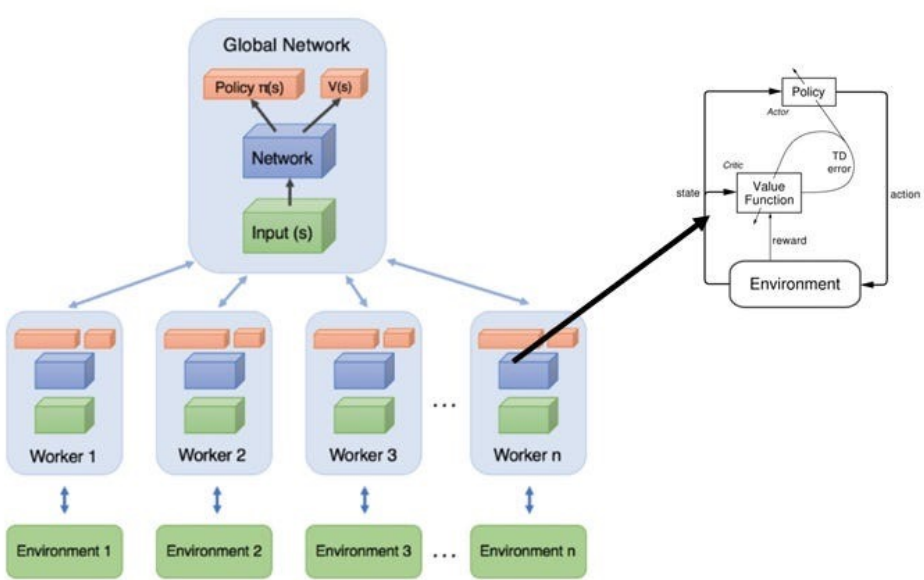
\includegraphics[width = \columnwidth]{
        figures/DeepReinforcementLearning3/A3C.png
    }
\end{figure}
Idea:
\begin{itemize}
    \item Use multiple workers
    \item Fixed length segments of experience to compute estimates of the return and advantage function
\end{itemize}
Asynchronous update:
\begin{itemize}
    \item Each agents updates the training network at its own time and independently
    \item Experience might come from older network copies of the other agents as well
    \item Data is uncorrelated, as the agents have different behaviors
    \item Allows on-policy training, which is more stable
\end{itemize}
\subsection{Advantage Actor-Critic (A2C)}
\begin{figure}[h!]
    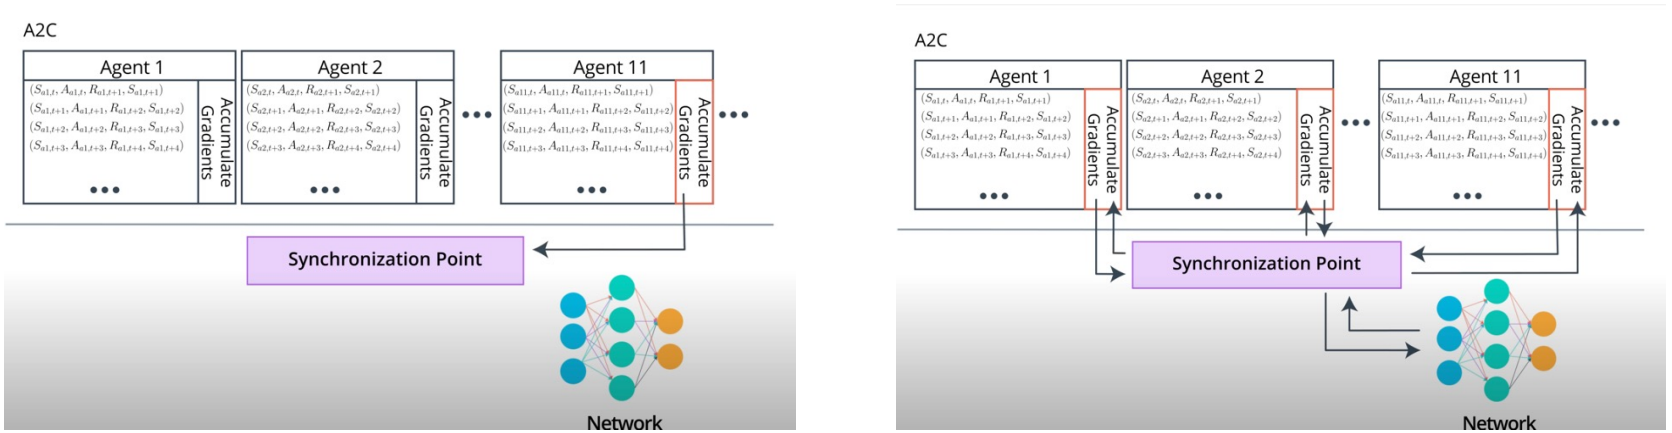
\includegraphics[width = \columnwidth]{
        figures/DeepReinforcementLearning3/A2C.png
    }
\end{figure}
Asynchronous doesnt improve performance.
It is also possible to use multiple workers, but wait until all workers have finished their episodes and then calculate an average gradient for the training step.